\documentclass[12pt, letterpaper]{article}
\usepackage{graphicx}
\usepackage[polish]{babel}
\usepackage[utf8]{inputenc}
\usepackage[T1]{fontenc}
\usepackage{mathpazo}

\graphicspath{{images/}}

%--------------------------------------------------------------------------------------------------
%       TITLE SECTION
%--------------------------------------------------------------------------------------------------
\begin{titlepage}

\begin{center}
	
\includegraphics[scale=0.2]{ur_inf_logo}\\ \\ \\ \\
\end{center}

\begin{center}

	\vspace{2cm}

	{Oskar Paśko}
	
	{117 987}
	
	{Informatyka i ekonometria} 
	
	\vspace{2cm}	
	
	{\textbf{Wykrywanie schorzeń daltonizmu za poomoca aplikacji VR}}
	
	\vspace{2cm}
	
	{\begin{flushright}
	Praca inżynierska
	
	\vspace{2cm}
	
	Praca wykonana pod kierunkiem \\
	
	\vspace{1cm}
	
	............................................
	\end{flushright}}
	
	\vspace{2cm}
	
	Rzeszów, 2023
\end{center}
\end{titlepage}

\usepackage{geometry}
 \geometry{
 a4paper,
 total={170mm,257mm},
 left=25mm,
 top=25mm,
 right=25mm,
 bottom=25mm 
 }
 
%--------------------------------------------------------------------------------------------------
%       BEGIN DOCUMENT
%--------------------------------------------------------------------------------------------------

\begin{document}
\setlength{\parindent}{1cm}
\newpage

%--------------------------------------------------------------------------------------------------
%       Streszczenie pracy (j.polskim) i tytuł pracy w języku angielskim
%--------------------------------------------------------------------------------------------------

\section{Streszczenie pracy}

%--------------------------------------------------------------------------------------------------
%       TABLE OF CONTENTS
%--------------------------------------------------------------------------------------------------
\tableofcontents

\newpage

%--------------------------------------------------------------------------------------------------
%       WPROWADZENIE
%--------------------------------------------------------------------------------------------------
\section{Wstęp}


\newpage
%--------------------------------------------------------------------------------------------------
%       ANALIZA AKTUALNEGO STANU WIEDZY O ZAGADNIENIU, KTÓREGO DOTYCZY PRACA
%--------------------------------------------------------------------------------------------------
\section{Analiza aktualnego stanu wiedzy o zagadnieniu, którego dotyczy praca}

\subsection{Daltonizm, czyli na czym polega zabuzenie rozpoznawania barw}

\paragraph{}
Daltonizm to zwyczajowa nazwa używana dla określenia dziedzicznego zaburzenia rozróżniania barw. Powodem, dla którego daltonista zmaga się z~nieprawidłowym widzeniem barw, jest brak lub osłabienie działania fotoreceptorów położonych na siatkówce oka, przede wszystkim w~obrębie plamki żółtej. Przyczyną dziedzicznego upośledzenia widzenia barwnego jest uszkodzenie genów kodujących odpowiednie barwniki wzrokowe.

%%%%%%%%%%%%%%%%%%%%%%%%%%%%%%%%%%
\subsection{Jak widzi daltonista?}

\paragraph{}
Daltonizm jest rodzajem wady wzroku i~nie jest tożsamy z~całkowitą ślepotą na barwy. Osoby z~tym schorzeniem zachowują widzenie barwy niebieskiej i~czerwonej. Nie rozpoznają koloru zielonego lub mylą go z~czerwonym. Czasami daltonista rozpoznaje barwę zieloną, ale bez postrzegania jej odcieni. Takie dyskretne zaburzenie widzenia określane jest mianem deuteranomalii.

\paragraph{}
Całkowita ślepota na barwy, czyli monochromatyzm to zdolność rozpoznawania tylko jednej barwy. Osoby z nieprawidłowością postrzegania barw mogą dostrzegać różnice w~kontraście, jaskrawości lub nasyceniu i~łączyć te cechy z~nazwami kolorów. W~rezultacie choroba ta może być zdiagnozowana dopiero w~życiu dorosłym. 

\begin{figure}[h]
  \centering
      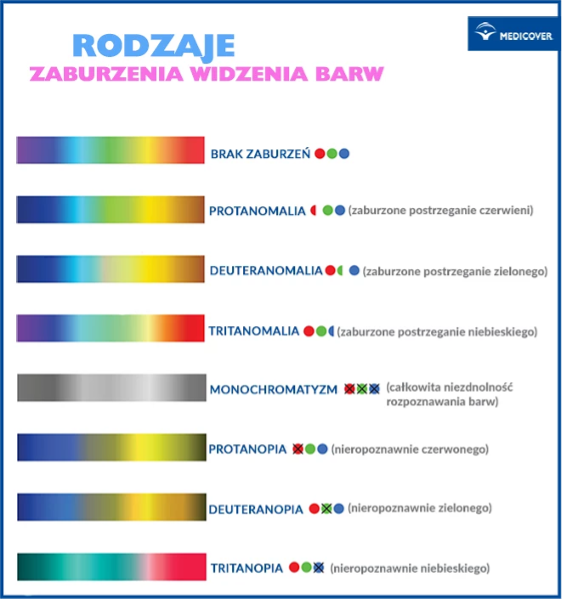
\includegraphics[width=0.6\textwidth]{daltonizm_rodzaje}
  \caption{Rodzaje zaburzeń widzenia barw}
\end{figure}

%%%%%%%%%%%%%%%%%%%%%%%%%%%%%%%%%%
\subsection{Testy na daltonizm}
\paragraph{}
Najpopularniejszym testem na daltonizm jest badanie z~wykorzystaniem pseudoizochromatycznych tablic Ishihary. Tablice te postać okrągłych plam złożonych z~kolorowych kropek, w~których ukryte są liczby lub określone kształty. Tablice te pozwalają na ocenę zaburzeń widzenia barwnego w~zakresie kolorów czerwonego i~zielonego. Badanie nie wymaga specjalnego przygotowania. Przeprowadza się je przy dobrym oświetleniu z~odległości umożliwiającej czytanie tekstu. Jeśli to konieczne osoba badana może założyć okulary.

\begin{figure}[h]
  \centering
      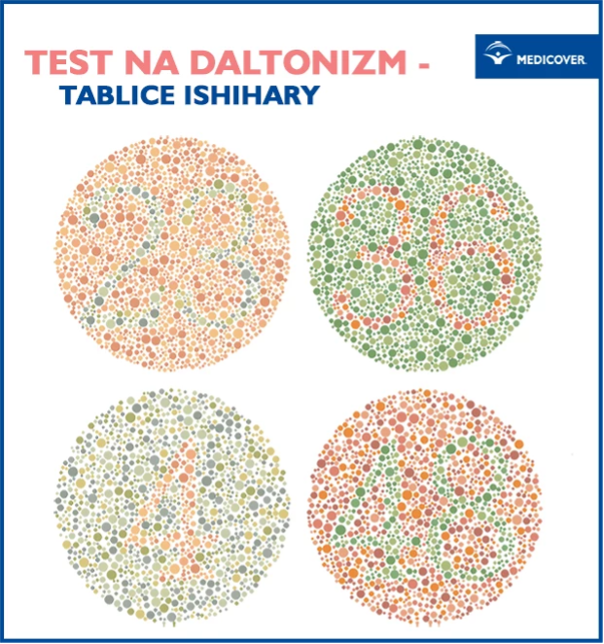
\includegraphics[width=0.7\textwidth]{ishihara}
  \caption{Tablice Ishihary}
\end{figure}

\paragraph{}
Odmiennym badaniem jest test Farnswortha D-15. Pozwala ocenić zdolność widzenia barwy czerwonej, zielonej i~niebieskiej. Polega na ułożeniu w~odpowiedniej kolejności 15 barwnych pionków tak, aby ich kolory płynnie przechodziły jeden w~drugi. W~przypadkach wątpliwych wykorzystuje się anomaloskop, czyli aparat służący do ilościowego określania zaburzenia widzenia barw w~osi czerwono-zielonej. Badanie ma przebieg dwufazowy. Najpierw zadaniem osoby badanej jest dobranie mieszaniny czystego światła czerwonego i~zielonego w~taki sposób, aby dopasować ją do czystego światła żółtego.

%--------------------------------------------------------------------------------------------------
%       SFORMUŁOWANIE ZAŁOŻEŃ I/LUB HIPOTEZ ORAZ NAKREŚLENIE CELU PRACY
%--------------------------------------------------------------------------------------------------

\section{Sformułowanie założeń i/lub hipotez oraz nakreślenie celu pracy}

%--------------------------------------------------------------------------------------------------
%       OMÓWIENIE METODYKI ORACY ORAZ UŻYTYCH URZĄDZEŃ I OPROGRAMOWANIE
%--------------------------------------------------------------------------------------------------

\section{Omówienie metodyki pracy oraz użytych urządzeń i oprgramowania}

\newpage

%--------------------------------------------------------------------------------------------------
%       OPIS ŚWIATA RZECZYWISTEGO
%--------------------------------------------------------------------------------------------------

\section{Opis świata rzeczywistego}

	\subsection{Opis zasobów ludzkich}

	Gra na urządzenia wirtualnej rzeczywistości takich jak Oculus Quest 2 polegająca na zabawie kolorami z~użyciem sześcianów lub innych obiektów na różnych planszach. Gra ma pomagać nad diagnozowaniem ewentualnych schorzeń daltonizmu lub jemu podobnych. Aplikacja może być również używana do zabawy rywalizacyjnej. Gra powinna być przystosowana dla użytkownika w~dowolnym wieku. Gra pozwala na zapisywanie za pomocą eye-trackera ścieżki wzroku z~jaką badany podążał podczas rozgrywki. Podczas rozgrywki mierzymy również czas wykonania zadania. Dzięki wynikom czasu, poprawności oraz ścieżkom eye-trackera jesteśmy w~stanie bardzo dobrze przeanalizować zachowanie gracza oraz stwierdzić podejrzenie schorzenia. Wszystkie wyniki oraz przebieg badań jest zapisywany w~postaci danych w~bazie danych, do której dostęp ma administrator.
	

	\subsection{Przepisy i strategia firmy}
	
	Strategią firmy jest pomoc dzieciom oraz osobom dorosłym w~diagnozowaniu schorzeń takich jak daltonizm itp. Dążymy do jak najlepszego kontaktu z~naszymi użytkownikami. Chcemy żeby nasi użytkownicy mieli jak największy wpływ na rozwój oprogramowania, które jest tworzone bezpośrednio dla nich. Przewidywane są częste aktualizacje oprogramowania w~celu poprawy działania aplikacji oraz dodawanie nowych funkcjonalności i~badań w~przyszłości. Aplikacja dodatkowo będzie wysyłać w~przeciągu tygodnia wyniki z~najnowszych badań razem z~ich interpretacją i~ewentualnymi zaleceniami. Dodatkowo priorytetem firmy będzie zadbanie o~bezpieczeństwo wrażliwych danych osobowych oraz danych konta naszych użytkowników.
	

	\subsection{Dane techniczne}
	
	Użytkownicy mogą korzystać z~aplikacji tylko na urządzeniach wirtualnej rzeczywistości. Użytkownicy mogą się zalogować do aplikacji tylko wtedy gdy mają połączenie z internetem. Jeśli użytkownik nie posiada konta może je darmowo utworzyć. Zarejestrowany użytkownik może się zalogować za pomocą unikatowego numeru telefonu oraz hasła. Aplikacja umożliwia kontakt z~administratorem w~celu weryfikacji oraz konsultacji przeprowadzonych badań.
	
%--------------------------------------------------------------------------------------------------
%       WYMAGANIA FUNKCJONALNE I NIEFUNKCJONALNE
%--------------------------------------------------------------------------------------------------

	\newpage	
	
	\subsection{Wymagania funkcjonalne i niefunkcjonalne}

		
			\begin{itemize}
				\item Logowanie do systemu za pomocą adresu email i hasła
				\item Możliwość zarejestrowania się do systemu
				\item Możliwość przeglądania historii badań
				\item Możliwość przeczytania opisów poszczególnych badań,
				\item Możliwość wyboru badań z listy,
				\item Wykonanie badania wybranego z listy,
			\end{itemize}
			
		
			\begin{itemize}
				\item Aplikacja zapewnia bezpieczeństwo wrażliwych danych,
				\item Aplikacja jest prosta w obsłudze,
				\item Aplikacja zapewnia schludny i przejrzysty interface,
				\item Aplikacja działa na urządzeniach wirtualnych Oculus Quest 2,
				\item Aplikacja jest tworzona w środowisku Unity,
				\item Aplikacja wykorzystuje bazę danych
			\end{itemize}
			
%--------------------------------------------------------------------------------------------------
%      	REQUREMENT DIAGRAM
%--------------------------------------------------------------------------------------------------
			
		\subsection{Requirement Diagram}
		
		W~oparciu o~opis świata rzeczywistego oraz zdefiniowane wymagania funkcjonalne i~niefunkcjonalne na Rys.1 przedstawiono diagram wymagań dla opisywanego oprogramowania.
		
\begin{figure}[h]
  \centering
      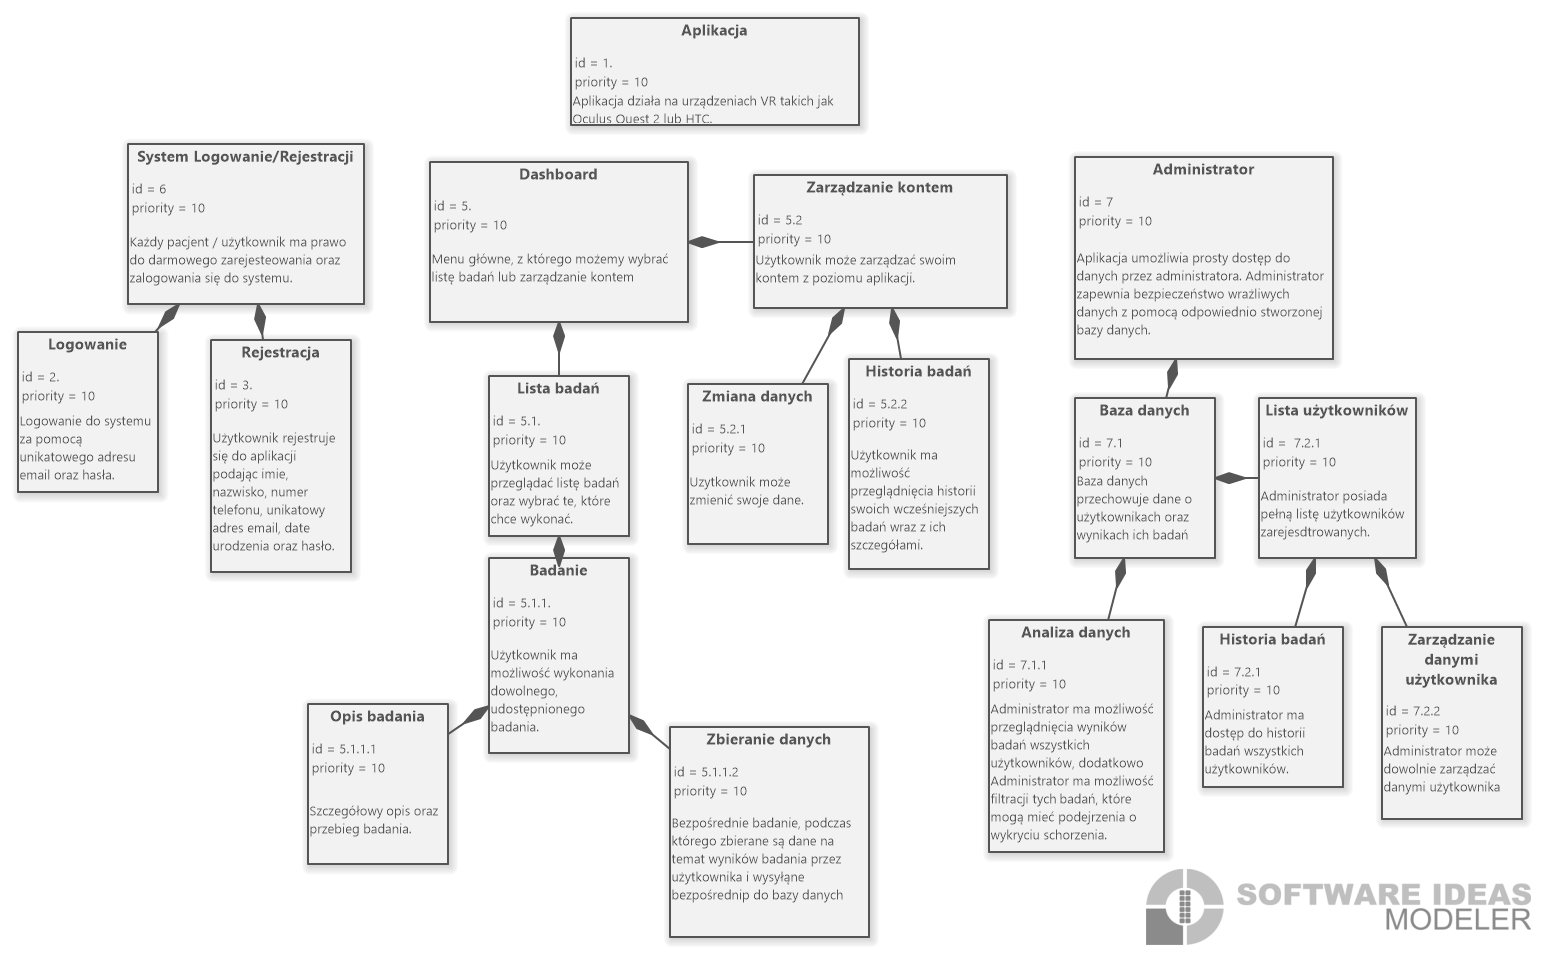
\includegraphics[width=0.8\textwidth]{reqDiagram}
  \caption{Diagram wymagań}
\end{figure}
		
		
\newpage
%--------------------------------------------------------------------------------------------------
%       DIAGRAMY UML
%--------------------------------------------------------------------------------------------------
		
		\section{Diagramy UML}

		W~tym rozdziale przedstawiona zostanie koncepcja projektowanego systemu za pomocą języka UML.		
		
		\subsection{Diagram przypadków użycia}
		
		W~oparciu o~opis świata rzeczywistego oraz zdefiniowane wymagania funkcjonalne i~niefunkcjonalne na Rys.2 przedstawiono diagram przypadków użycia dla opisywanego oprogramowania.

\begin{figure}[h]
  \centering
      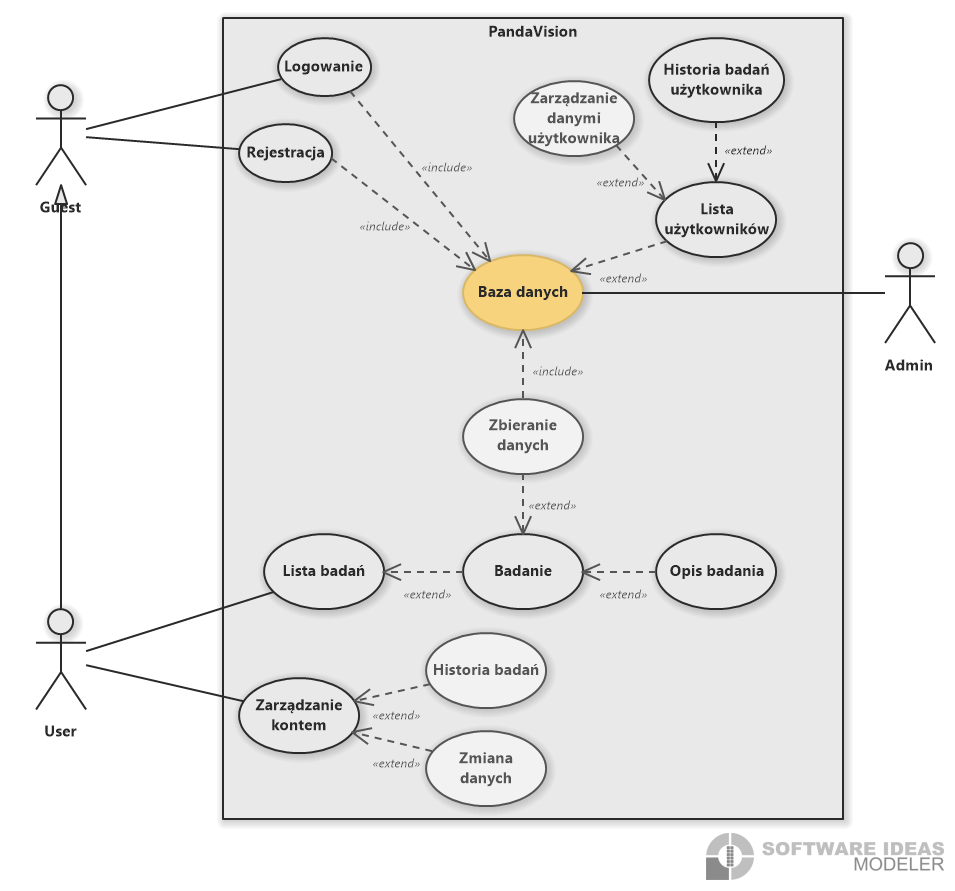
\includegraphics[width=0.8\textwidth]{useCaseDiagram}
  \caption{Diagram przypadków użycia}
\end{figure}			
		
		
%--------------------------------------------------------------------------------------------------
%       DEFINICJA AKTORÓW
%--------------------------------------------------------------------------------------------------

		\newpage		
		
		\textbf{Definicje scenariuszy przypadków użycia} (PU - przypadek użycia, WS - warunki wstępne, WK - warunki końcowe)\\
		
		\quad		
		
		\textbf{Aktor:} Gość\\
		
		\textbf{Opis:} Gość może się zalogować lub zarejestrować do systemu.\\
		
		\textbf{Przypadki użycia:} PU Logowanie, PU Rejestracja.
		
		\vspace{1cm}
		
		\textbf{Aktor:} Użytkownik\\
		
		\textbf{Opis:} Użytkownik oprócz funkcjonalności gości może przeglądać listę badań, opisy badań oraz historie swoich badań. Użytkownik może również zacząć dowolne badanie dostępne z~listy.\\
		
		\textbf{Przypadki użycia:} PU Lista badań, PU Zarządzanie kontem, PU Edycja danych powiązane przez << extend >> z~PU Zarządzanie kontem, PU Historia badań powiązane przez << extend >>\\ z~PU Zarządzanie kontem, PU Opis badania powiązane przez << extend >> z~PU Lista badań,\\ PU Start powiązane przez << extend >> z~PU Lista badań. 
		
		\vspace{1cm}
		
		\textbf{Aktor:} Administrator\\
		
		\textbf{Opis:} Administrator zarządza systemem, bazą danych oraz analizuje wyniki badań użytkowników.\\
		
		\textbf{Przypadki użycia:} PU Baza danych, PU Zarządzanie systemem, PU Historia badań użytkownika powiązane przez << extend >> z~PU Zarządzanie systemem, PU Zarządzanie danymi użytkownika powiązane przez << extend >> z~PU Zarządzanie systemem.	

		
%-------------------------------------------
%       PU BAZA DANYCH
%-------------------------------------------	
		
		\textbf{PU Baza danych}
		
		\quad
		
		\textbf{Cel: Zarządzanie danymi}\\
		
		WS: Rest API.\\
		
		WK: Możliwość zarządzania danymi.\\
		
		\textbf{Przebieg: }\\
		Baza danych będzie wykorzystywana do możliwości logowania oraz rejestracji. Ponadto będą się w~niej znajdować wyniki badań użytkowników. Baza danych będzie się składać z~tabeli przechowujących dane użytkowników takie jak adres e-mail, imię, nazwisko, hasło, numer telefonu oraz datę urodzenia. Ponadto baza danych będzie posiadać tabelę z~badaniami, w~której będą zamieszczone wszystkie niezbędne dane dotyczące badań takie jak czas wykonania badania, datę przeprowadzenia badania, pliki zebrane podczas badania np. ścieżka eye-trackera oraz informację, który użytkownik przeprowadził konkretne badanie.
		 \\
		
		
%-------------------------------------------
%       PU LOGOWANIE
%-------------------------------------------	
		
		\textbf{PU Logowanie}
		
		\quad
		
		\textbf{Cel: Zalogowanie do systemu}\\
		
		WS: może być wywołany z PU Logowanie.\\
		
		WK: podanie niezbędnych danych do zalogowania tj. adres e-mail i hasło.\\
		
		\textbf{Przebieg:}\\
		Logowanie dostępne jest poprzez zakładkę "Logowanie". Podczas logowania należy podać adres e-mail oraz hasło. W~przypadku podania błędnych danych pojawi się informacja o~niepowodzeniu logowania w~postaci komunikatu "Podano błędne dane". Użytkownik może ponownie podać dane lub wyjść z~aplikacji. W~przypadku 5 błędnych logowań system zablokuje konto i~wyświetli komunikat "Prosimy o~kontakt w~celu odblokowania konta". Jeśli użytkownik wprowadzi poprawne dane to użytkownik zostanie zalogowany do systemu i~przeniesie się automatycznie do panelu głównego aplikacji.\\
		
%-------------------------------------------
%       PU REJESTRACJA
%-------------------------------------------	
		
		\newpage		
		
		\textbf{PU Rejestracja}
		
		\quad
		
		\textbf{Cel: Rejestracja do systemu}\\
		
		WS: może być wywołany z PU Rejestracja.\\
		
		WK: podanie niezbędnych danych do zalogowania tj. imię, nazwisko, adres e-mail, hasło, numer telefonu, data urodzenia.\\
		
		\textbf{Przebieg:}\\
		Rejestracja jest dostępna przez zakładkę "Rejestracja". Podczas rejestracji należy podać imię, nazwisko, datę urodzenia, numer telefonu, unikalny adres e-mail oraz hasło. W~przypadku podania niewłaściwych danych np. numeru telefonu o~długości 10 cyfr lub adresu e-mail bez znaku "@" wyskoczy komunikat "Wprowadzono nieprawidłowe dane". W przypadku podania adresu e-mail, który już jest przypisany do innego konta wyskoczy komunikat "Konto z~podanym adresem e-mail już istnieje". Użytkownik może ponownie podać dane lub wyjść z aplikacji. Jeśli użytkownik wprowadzi poprawne dane to zostanie przekierowany do panelu logowania, gdzie będzie mógł się zalogować odpowiednimi danymi. \\
		
%-------------------------------------------
%       PU LISTA BADAŃ
%-------------------------------------------	
		
		\textbf{PU Lista badań}
		
		\quad
		
		\textbf{Cel: Wybór badania z listy}\\
		
		WS: może być wywołany z PU Lista badań.\\
		
		WK: wybór badania z listy\\
		
		\textbf{Przebieg:}\\
		Lista badań jest dostępna przez zakładkę "Lista badań". Użytkownik może przeglądać dostępne badania, które są zaprezentowane w~postaci listy za pomocą nazw badań oraz dwóch przycisków "Start oraz "Opis". Po kliknięciu przycisku "Opis" użytkownik zostanie wyświetlony opis badania. Po kliknięciu w przycisk "Start" użytkownik zacznie wybrane badanie. \\
		
%-------------------------------------------
%       PU START
%-------------------------------------------	
		
		\textbf{PU Start}
		
		\quad
		
		\textbf{Cel: Zaznajomienie się z badaniem}\\
		
		WS: może być wywołany z PU Start.\\
		
		WK: wykonanie badania.\\
		
		\textbf{Przebieg: }\\
		Badanie możemy wywołać po wybraniu odpowiedniego badania z listy. Podczas badania będą zbierane dane z przeprowadzanego badania takie jak czas, wynik lub ścieżka wzroku, liczba popełnionych błędów. Po zakończeniu badania, wszystkie dane są zapisywane w~bazie danych zgodnie z~metodologią zapisu plików.
		 \\
		 
%-------------------------------------------
%       PU OPIS BADANIA
%-------------------------------------------	
		
		\textbf{PU Opis Badania}
		
		\quad
		
		\textbf{Cel: Zaznajomienie się z przebiegiem badania}\\
		
		WS: może być wywołany z PU badania.\\
		
		WK: zaznajomienie się z przebiegiem badania.\\
		
		\textbf{Przebieg: }\\
		Użytkownik będzie mógł przeczytać szczegółowy opis na temat konkretnego badania oraz przeczytać szczegółowy przebieg badania. Dostępne będą również przykładowe zrzuty ekranu z~przebiegu badania.
		 \\
		 
%-------------------------------------------
%       PU ZARZĄDZANIE KONTEM
%-------------------------------------------	
		
		\textbf{PU Zarządzanie kontem}
		
		\quad
		
		\textbf{Cel: Zarządzanie danymi}\\
		
		WS: może być wywołany z PU Zarządzanie kontem.\\
		
		WK: zarządzanie danymi.\\
		
		\textbf{Przebieg:}\\
		Użytkownik może wybrać zakładkę "Historia badań" lub zakładkę "Zmiana danych" za pomocą, których będzie mógł zarządzać swoimi danymi lub historią swoich badań.
		 \\
		 
%-------------------------------------------
%       PU HISTORIA BADAŃ
%-------------------------------------------	
		
		\textbf{PU Historia badań}
		
		\quad
		
		\textbf{Cel: Przeglądanie historii badań}\\
		
		WS: może być wywołany z PU Historia badań.\\
		
		WK: przeglądanie historii badań.\\
		
		\textbf{Przebieg:}\\
		Użytkownik może przeglądać listę z~historią swoich badań reprezentowaną nazwą badania oraz datą. Po kliknięciu w~badanie rozwinie się zakładka z~szczegółowymi danymi dotyczącymi konkretnego badania.
		 \\
		 
%-------------------------------------------
%       PU ZMIANA DANYCH
%-------------------------------------------	
		
		\newpage		
		
		\textbf{PU Zmiana danych}
		
		\quad
		
		\textbf{Cel: Możliwość zmiany danych personalnych}\\
		
		WS: może być wywołany z PU Zmiana danych.\\
		
		WK: możliwość zmiany danych personalnych.\\
		
		\textbf{Przebieg:}\\
		Użytkownik będzie mógł zmienić dane. Aktualne dane zostaną wpisane w~wierze. Użytkownik będzie mógł zmienić dowolne dane oraz zaakceptować zmiany przez wciśnięcie przycisku "Aktualizuj". Po wciśnięciu przycisku nastąpi walidacja nowych danych oraz zapis do bazy danych.
		 \\
			
		
%-------------------------------------------
%       PU  ZARZĄDZANIE SYSTEMEM
%-------------------------------------------	
		
		\textbf{PU Zarządzanie systemem}
		
		\quad
		
		\textbf{Cel: Zarządzanie bazą danych}\\
		
		WS: może być wywołany z PU Zarządzanie systemem.\\
		
		WK: zarządzanie bazą danych. \\
		
		\textbf{Przebieg:}\\
		Jeśli administrator prawidłowo zaloguje się do systemu to zostaje wyświetlona w~panelu głównym lista użytkowników zarejestrowanych do systemu w~postaci listy. Lista jest reprezentowana za pomocą imienia, nazwiska oraz adresu e-mail użytkownika. Klikając w użytkownika z~listy możemy przejść do szczegółów jego konta.\\	
		
%-------------------------------------------
%       PU HISTORIA BADAŃ UŻYTKOWNIKA
%-------------------------------------------	
		
		\textbf{PU Historia badań użytkownika}
		
		\quad
		
		\textbf{Cel: Przeglądanie historii badań użytkownika}\\
		
		WS: może być wywołany z PU Historia badań użytkownika.\\
		
		WK: przeglądanie historii badań użytkownika. \\
		
		\textbf{Przebieg:}\\
		Po wybraniu użytkownika z~listy administrator zobaczy listę badań konkretnego użytkownika. Wyświetlane będą takie informacje jak: data badania, rodzaj badania oraz wyniki badań, dodatkowo powinny być pokazane pliki do pobrania, które stworzyły się podczas badania jak np. ścieżka śledzenia wzroku lub wykresy danych dostarczonych podczas badania. W~przypadku stwierdzenia podejrzenia schorzenia poprzez nieprawidłowości związane z~badaniem administrator przez zakładkę "Kontakt" powinien mieć bezpośrednią możliwość wysłania na adres e-mail użytkownika informacji na temat wyników badania wraz z~udostępnieniem wszelkich danych oraz plików.
		
%-------------------------------------------
%       PU ZARZĄDZANIE DANYMI UŻYTKOWNIKA
%-------------------------------------------	
		
		\newpage		
		
		\textbf{PU Zarządzanie danymi użytkownika}
		
		\quad
		
		\textbf{Cel: Zmiana danych personalnych}\\
		
		WS: może być wywołany z PU Zarządzanie danymi użytkownika.\\
		
		WK: zmiana danych personalnych.\\
		
		\textbf{Przebieg:}\\
		Administrator ma możliwość odblokowania konta użytkownika oraz ewentualną zmianę danych użytkownika. Ponadto administrator ma dostęp do wszystkich szczegółowych danych związanych z~badaniami użytkownika.
		 \\
		

		

%--------------------------------------------------------------------------------------------------
%       DIAGRAM AKTYWNOŚCI
%--------------------------------------------------------------------------------------------------
		\subsection{Diagram aktywności}
		
		W oparciu o~diagram przypadków użycia oraz przebiegu PU Logowanie i~PU Rejestracja na Rys.3 oraz Rys.4 przedstawiono kolejno diagram aktywności logowania i~diagram aktywności rejestracji dla opisywanego oprogramowania.
		
\begin{figure}[h]
  \centering
      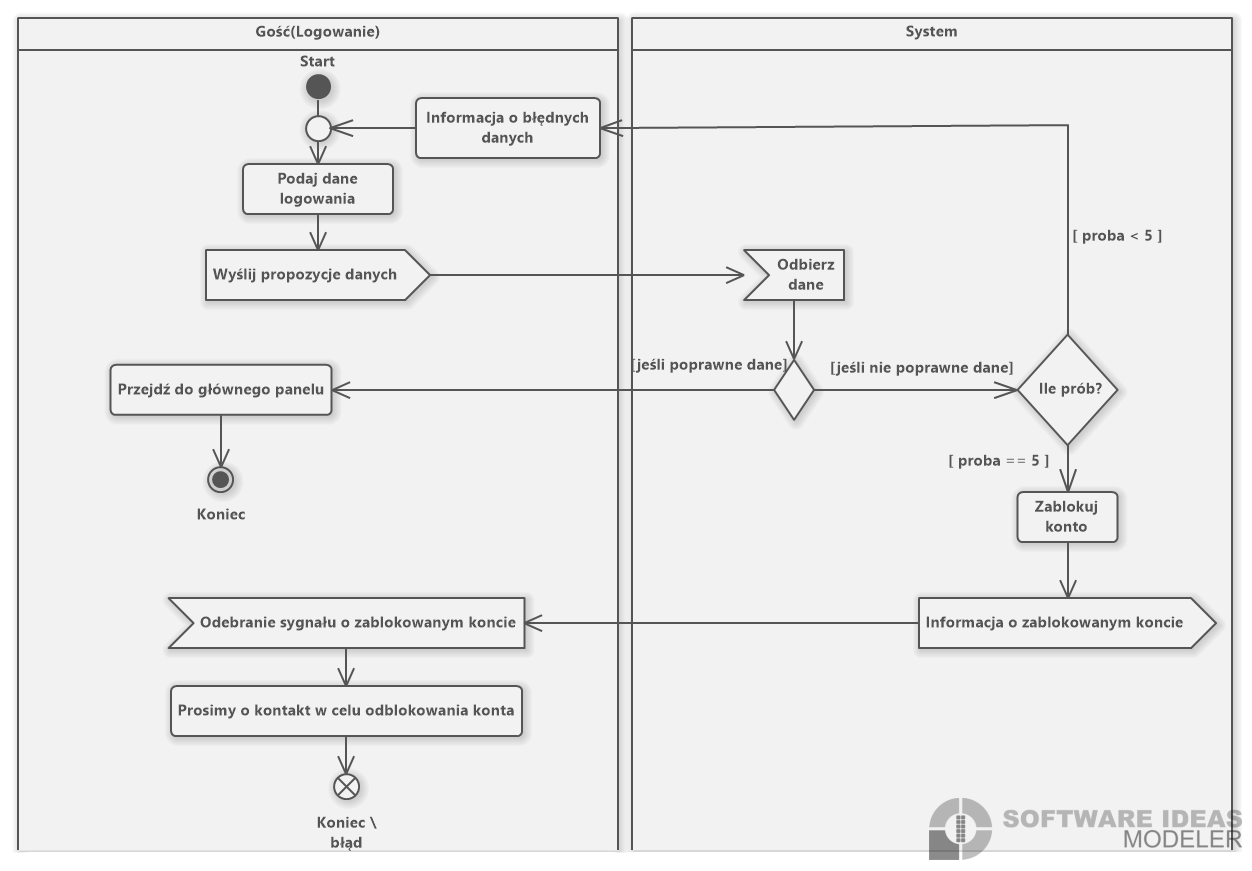
\includegraphics[width=0.8\textwidth]{aclogowanie}
  \caption{Diagram aktywności - Logowanie}
\end{figure}

\begin{figure}[h]
  \centering
      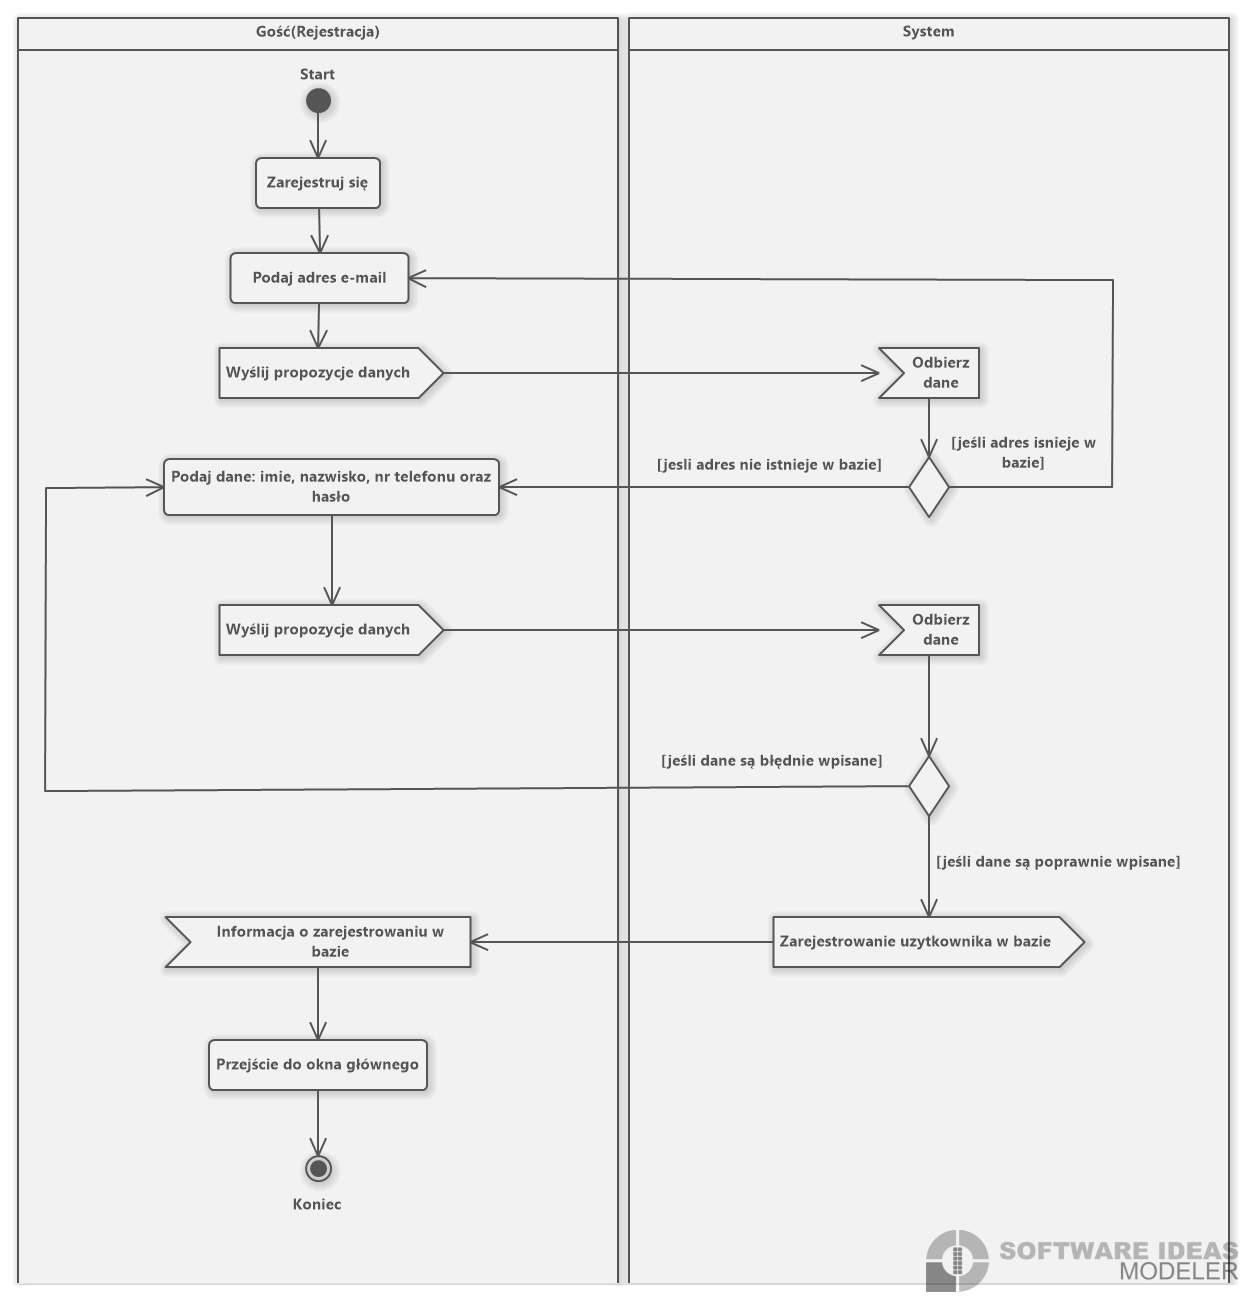
\includegraphics[width=0.8\textwidth]{acrejestracja}
  \caption{Diagram aktywności - Rejestracja}
\end{figure}
		
		
\newpage
%--------------------------------------------------------------------------------------------------
%       DIAGRAM KLAS
%--------------------------------------------------------------------------------------------------
		\subsection{Diagram klas}
		
		Na podstawie diagramu przypadków użycia na Rys.5 przedstawiono diagram klas dla opisywanego oprogramowania.\\	
		
		Klasa {\fontfamily{qcr}\selectfont BazaDanych} odpowiedzialna jest za połączenie z~bazą danych. Główna klasa {\fontfamily{qcr}\selectfont Start}, będzie wywoływana podczas uruchamiania aplikacji. Klasa będzie tworzyć instancje klas Logowanie lub Rejestracja w~zależności od wyboru użytkownika. Klasa {\fontfamily{qcr}\selectfont Logowanie} będzie odpowiedzialna za system logowania do aplikacji. Klasa będzie korzystać z~klasy BazaDanych. Klasa będzie się znajdować w~klasie Start oraz tworzyć instancję klasy Uzytkownik, jeśli nastąpi poprawne logowanie do systemu. Klasa {\fontfamily{qcr}\selectfont Rejestracja} odpowiedzialna będzie za rejestrowanie użytkownika do systemu oraz walidacji danych podczas rejestracji. Klasa będzie korzystać z~klasy BazaDanych oraz będzie znajdować się w~klasie Start. Klasa {\fontfamily{qcr}\selectfont Osoba} będzie klasą abstrakcyjną, po której będzie dziedziczyć klasa reprezentująca użytkowników. Klasa {\fontfamily{qcr}\selectfont Uzytkownik} dziedziczy po klasie Osoba oraz zawiera składowe takie jak numer pacjenta oraz imię. Klasa zawiera metody, które będą wykorzystane do reprezentowania danych użytkownika oraz przekazywania numeru pacjenta do innych klas. Klasa {\fontfamily{qcr}\selectfont Dashboard} będzie odpowiedzialna za obsługę menu głównego użytkownika. Klasa ta będzie tworzyć instancje klas ListaBadan lub Konto. Klasa {\fontfamily{qcr}\selectfont Konto} odpowiedzialna będzie za zarządzanie przez użytkownika swoimi danymi. Klasa będzie połączona z~klasą BazaDanych oraz będzie się znajdować w~klasie Dashboard. Klasa {\fontfamily{qcr}\selectfont Badanie} to klasa, która zawiera wszystkie składowe danego badania oraz metody sterujące badaniem. Ponadto klasa zawiera główną metodę start(), która rozpoczyna badanie oraz metodę opis(), która wyświetli szczegółowy opis badania. Klasa ta będzie wywoływana w klasie ListaBadan. Klasa {\fontfamily{qcr}\selectfont ListaBadan} będzie tworzyć posortowaną listę klas z~dostępnymi badaniami. Klasa będzie również umożliwiać otworzenie opisu danego badania lub jego rozpoczęcie za pomocą metod start() oraz opis() z klasy Badanie.\\
		
\begin{figure}[h]
  \centering
      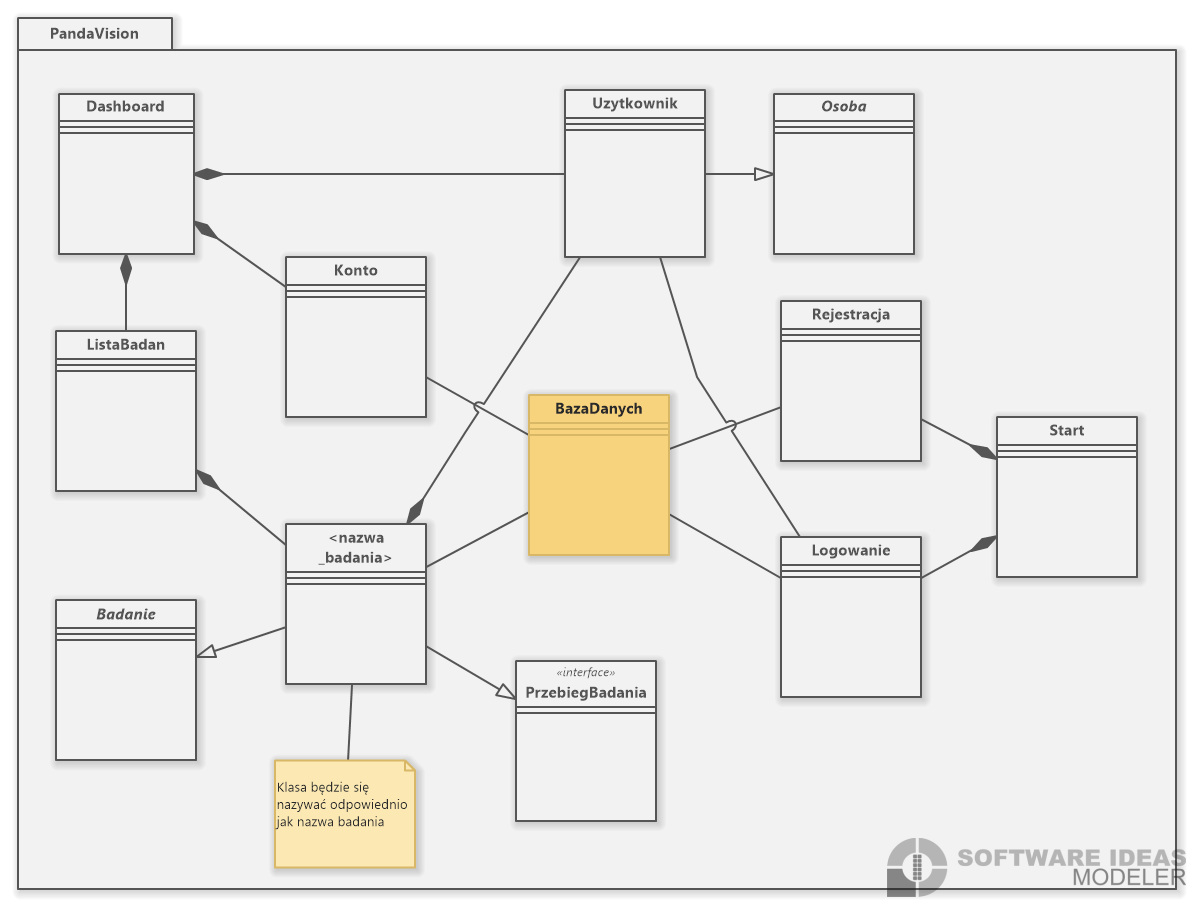
\includegraphics[width=0.8\textwidth]{classDiagram}
  \caption{Diagram klas}
\end{figure}
		
		
%--------------------------------------------------------------------------------------------------
%       DIAGRAM SEKWENCJI
%--------------------------------------------------------------------------------------------------
		\newpage

		\subsection{Diagram sekwencji}
		
		Na podstawie diagramów aktywności logowania oraz rejestracji na Rys.6 oraz Rys.7 przedstawiono kolejno diagram sekwencji logowania oraz diagram sekwencji rejestracji dla opisywanego oprogramowania.
		
\begin{figure}[h]
  \centering
      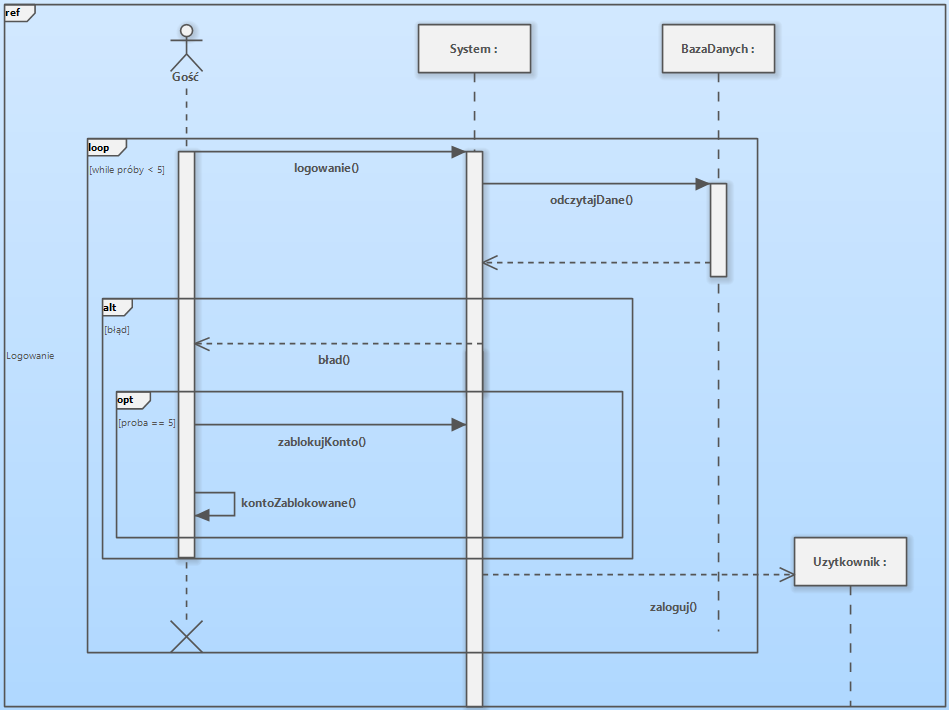
\includegraphics[width=0.8\textwidth]{seqDiagram}
  \caption{Diagram sekwencji - Logowanie}
\end{figure}

\begin{figure}[h]
  \centering
      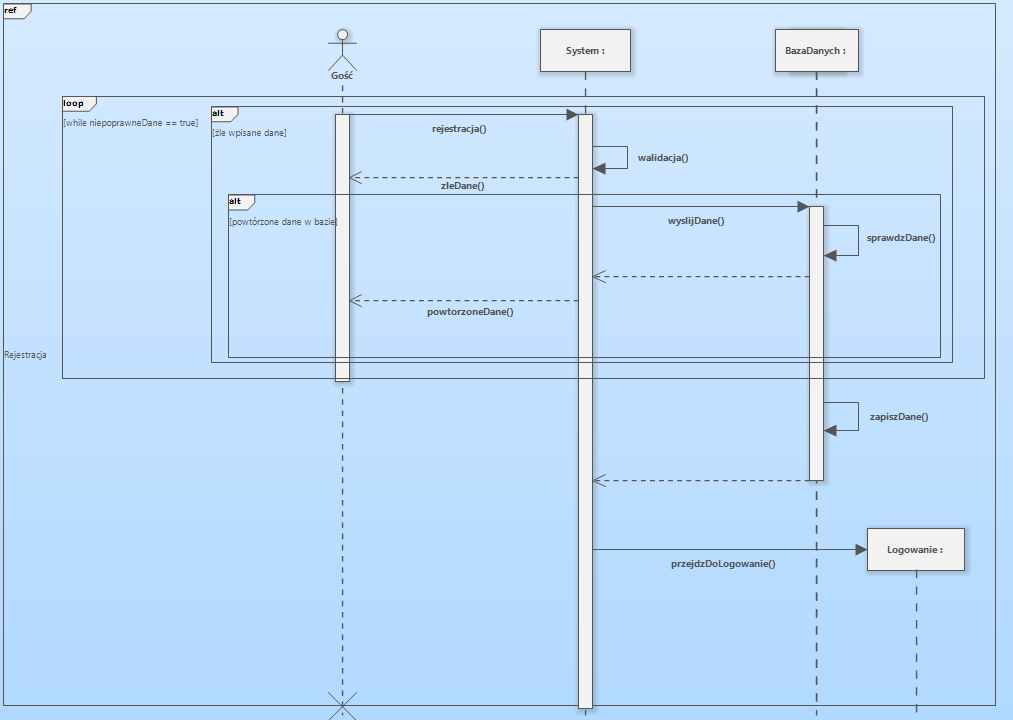
\includegraphics[width=0.8\textwidth]{seqDiagramRejestracja}
  \caption{Diagram sekwencji - rejestracja}
\end{figure}
		
%--------------------------------------------------------------------------------------------------
%       DIAGRAM AKTYWNOŚCI
%--------------------------------------------------------------------------------------------------
		\newpage		
		
		\subsection{Diagram stanów}
		
		Na podstawie diagramów aktywności logowania oraz rejestracji na Rys.8 przedstawiono diagram stanów z~cyklu życia obiektu Uzytkownik w~aplikacji.\\
		
		Nowy użytkownik może się zarejestrować, a~następnie staje się Zarejestrowany. Po zarejestrowaniu się, użytkownik może przystąpić do próby logowania do systemu. Jeśli użytkownik wpisze poprawne dane zostanie zalogowany i~stanie się Zalogowany. Zalogowany użytkownik może się w~dowolnym momencie wylogować z~systemu i~stanie się znowu Zarejestrowany. Jeśli podczas próby logowania użytkownik poda 5 razy złe dane konto zostanie zablokowane i~stanie się Zablokowany. Użytkownik może poprosić administratora o~odblokowanie konta. Po odblokowaniu konta użytkownik stanie się znowu Zarejestrowany.
		
\begin{figure}[h]
  \centering
      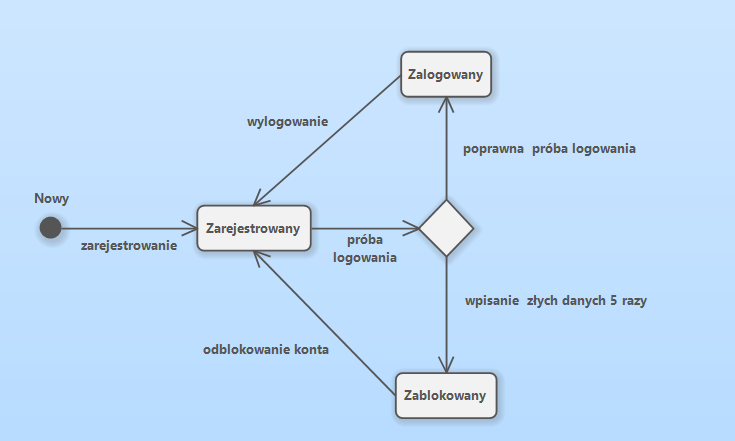
\includegraphics[width=0.8\textwidth]{activeDiagramUser}
  \caption{Diagram stanów użytkownika}
\end{figure}
		
		
%--------------------------------------------------------------------------------------------------
%       HARMONOGRAM REALIZACJI PROJEKTU
%--------------------------------------------------------------------------------------------------
		\newpage
		\section{Harmonogram realizacji projektu}
		
		Poniżej zamieszczono harmonogram realizacji projektu. Diagram Gantta prezentuje ilość dni jakie będą poświęcone poszczególnym pracom oraz suma dni spędzonych podczas pracy nad projektem.
		
\begin{figure}[h]
  \centering
      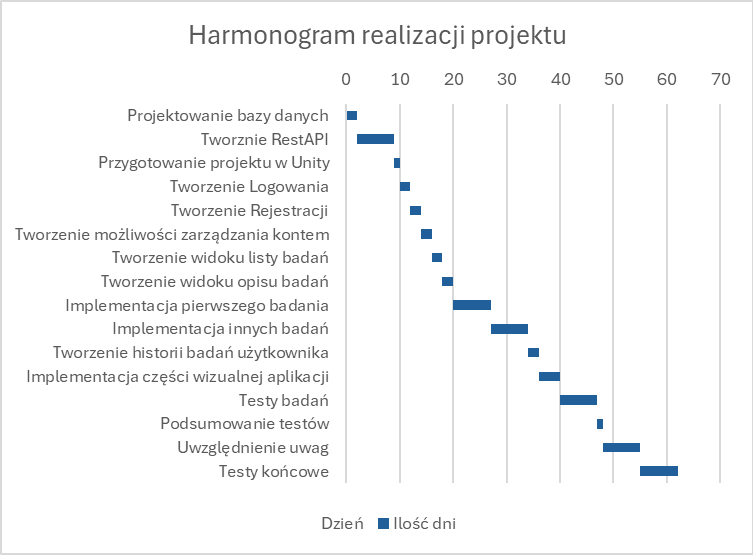
\includegraphics[width=0.6\textwidth]{wykres_gantta}
  \caption{Wykres Gantta}
\end{figure}
		
		
%--------------------------------------------------------------------------------------------------
%       OPIS TECHNICZNY PROJEKTU
%--------------------------------------------------------------------------------------------------
		\section{Opis techniczny projektu}
		
		\begin{itemize}
				\item Środowisko programistyczne VR: Unity 2023.2.51
				\item Środowisko programistyczne Flask: PyCharm 2023.3
				\item Aplikacja jest projektowana na urządzenia wirtualnej rzeczywistości takie jak - Oculus Quest 2, HTC Vive
		\end{itemize}
			
%--------------------------------------------------------------------------------------------------
%       INTERFEJS UŻYTKOWNIKA
%--------------------------------------------------------------------------------------------------
		\newpage
		\section{Interfejs użytkownika}
		
		Na Rys.10 przedstawiono koncepcję tablicy jaką zobaczy użytkownik po wejściu do aplikacji. Użytkownik będzie mógł:
		\begin{itemize}
				\item Zalogować się wciskając przycisk "Zaloguj" po wprowadzeniu poprawnych danych;
				\item Przejść do formularza rejestracji wciskając przycisk "Zarejestruj"
				\item Przypomnieć hasło poprzez wciśnięcie przycisku "Kliknij tutaj"
		\end{itemize}
		
\begin{figure}[h]
  \centering
      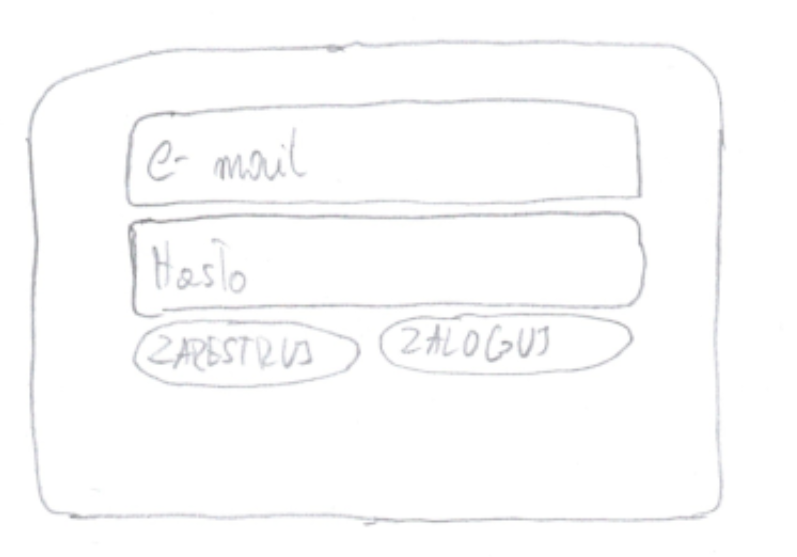
\includegraphics[width=0.5\textwidth]{GUI_logowanie}
  \caption{Formularz logowania do aplikacji}
\end{figure}
	
		
		Na Rys.11 przestawiono koncepcję tablicy jaką zobaczy użytkownik po wejściu do możliwości rejestracji. Użytkownik będzie mógł się zarejestrować do systemu wprowadzając poprawne dane oraz wciskając przycisk "Zarejestruj".
		
\begin{figure}[h]
  \centering
      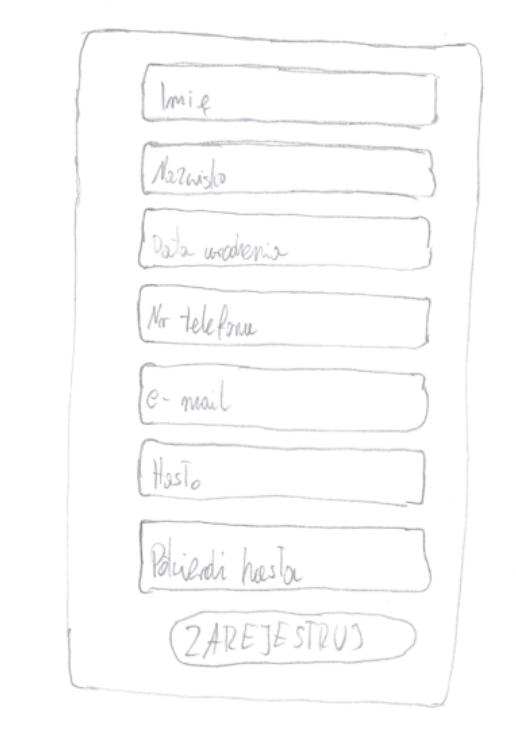
\includegraphics[width=0.5\textwidth]{GUI_rejestracja}
  \caption{Formularz rejestracji do aplikacji}
\end{figure}
		
		Na Rys.12 przedstawiono koncepcję tablicy z~listą badań jaką użytkownik zobaczy wchodząc w~scenę z~listą badań. Użytkownik będzie mógł:
		
		\begin{itemize}
			\item Przeglądać dostępne badania;
			\item Zacząć badanie po wciśnięciu przycisku "Start";
			\item Przeczytać opis wchodząc do oddzielnej sceny poprzez przycisk "Opis"
		\end{itemize}
		
\begin{figure}[h]
  \centering
      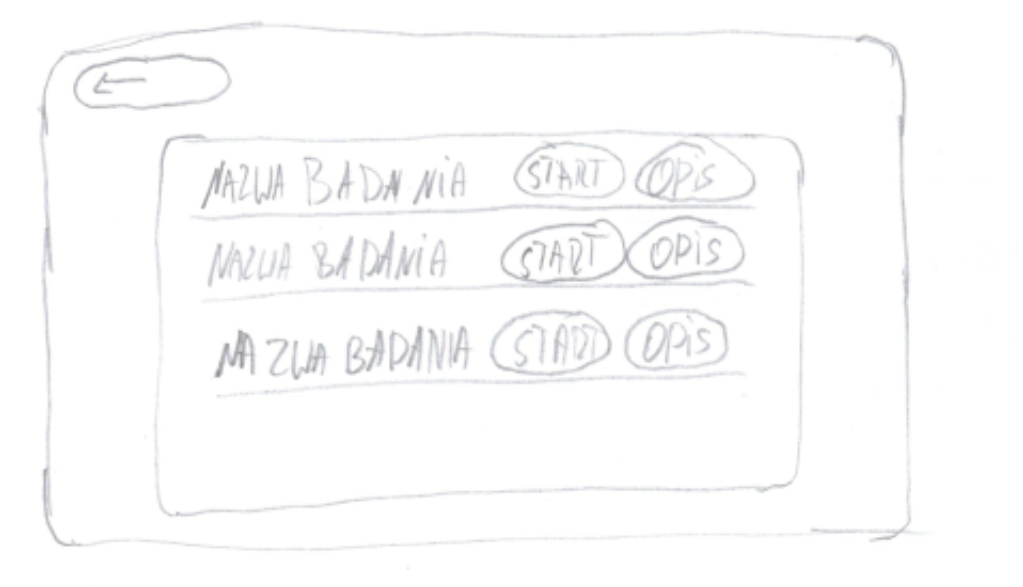
\includegraphics[width=0.5\textwidth]{GUI_lista_badan}
  \caption{Tablica z listą badań}
\end{figure}
		
		Na Rys.13 przedstawiono koncepcję tablicy z~opisem badania, którą użytkownik zobaczy po wciśnięciu przycisku "Opis" w~scenie z~listą badań. Użytkownik będzie mógł przeczytać szczegółowy opis badania oraz przeglądnąć przykładowe zrzuty ekranu z przebiegu badania, które będą umieszczone pod opisem słownym.
		
\begin{figure}[h]
  \centering
      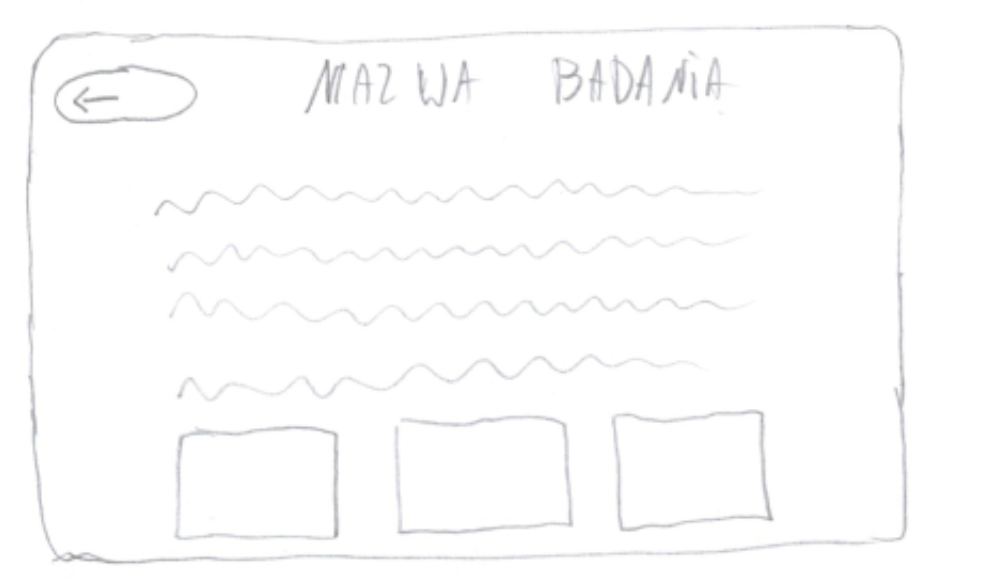
\includegraphics[width=0.5\textwidth]{GUI_opis_badania}
  \caption{Tablica z opisem badania}
\end{figure}
		
		Na Rys.14 przedstawiono koncepcję tablicy z~dwoma kafelkami do zarządzania kontem. Użytkownik będzie mógł:
		
		\begin{itemize}
			\item Przejść do historii swoich badań za pomocą przycisku "Historia badań"
			\item Przejść do zarządzania swoimi danymi za pomocą przycisku "Zarządzaj kontem"
		\end{itemize}

		
\begin{figure}[h]
  \centering
      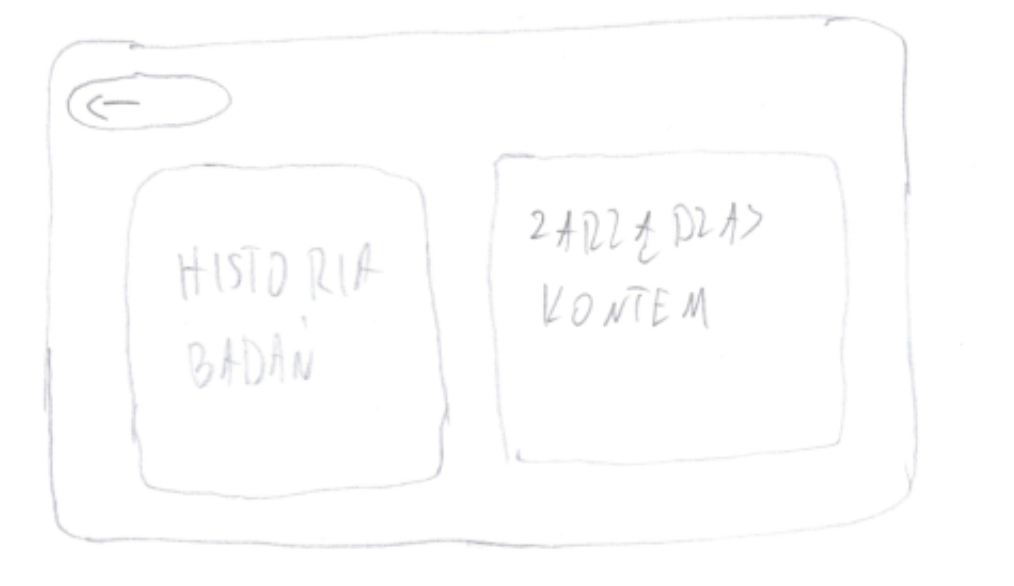
\includegraphics[width=0.5\textwidth]{GUI_zarzadzanie_kontem}
  \caption{Tablica z zarządzaniem kontem}
\end{figure}
		
		Na Rys.15 przedstawiono koncepcję tablicy z historią badań. Użytkownik będzie mógł przeglądać  swoją historię badań. Badania są wyświetlane za pomocą nazwy danego badania oraz daty jego wykonania. Po wciśnięciu dowolnego badania rozwinie się okienko ze szczegółowymi danymi.
		
\begin{figure}[h]
  \centering
      \includegraphics[width=0.5\textwidth]{GUI_istoroa_badan}
  \caption{Tablica z historią badań}
\end{figure}
		
		Na Rys.16 przedstawiono formularz dzięki któremu użytkownik może zmienić swoje dane. Użytkownik może wprowadzić na miejsce starych danych nowe dane. Po wciśnięciu przycisku "Aktualizuj" następuje walidacja danych oraz zapis nowych wartości do bazy danych.
		
\begin{figure}[h]
  \centering
      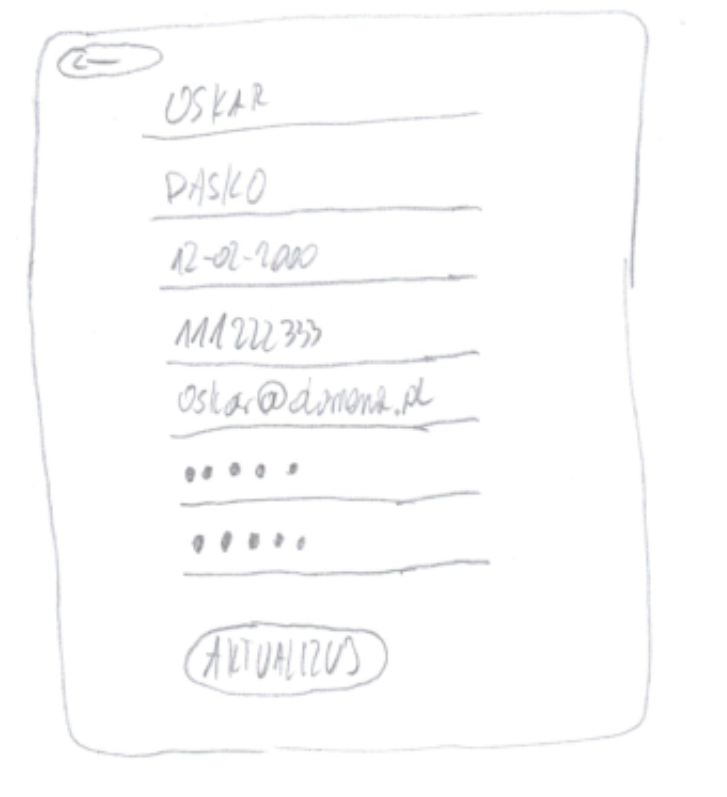
\includegraphics[width=0.5\textwidth]{GUI_zmiana_danych}
  \caption{Formularz aktualizujący dane}
\end{figure}
		
%--------------------------------------------------------------------------------------------------
%       PODSUMOWANIE
%--------------------------------------------------------------------------------------------------

		\section{Podsumowanie}
		
		Aplikacja jest projektowania z~myślą o~osobach zmagającymi się ze schorzeniami daltonizmu. Oprogramowanie będzie miało za zadanie ułatwienie rozpoznawania schorzeń dotyczących daltonizmu u~dzieci przez zabawę oraz gry w~aplikacji. Chcemy połączyć gry i~zabawy razem z~badaniami wzroku. Chcemy żeby dzieci podczas badania czuły się jakby grały lub rywalizowały z~wynikami poprzedników. Nie chcemy żeby skupiały się na myśli, że są badane aby oszczędzić im niepotrzebnego stresu oraz zdenerwowania wynikami.
 
\end{document}
